\documentclass[]{article}
\usepackage{lmodern}
\usepackage{amssymb,amsmath}
\usepackage{ifxetex,ifluatex}
\usepackage{fixltx2e} % provides \textsubscript
\ifnum 0\ifxetex 1\fi\ifluatex 1\fi=0 % if pdftex
  \usepackage[T1]{fontenc}
  \usepackage[utf8]{inputenc}
\else % if luatex or xelatex
  \ifxetex
    \usepackage{mathspec}
  \else
    \usepackage{fontspec}
  \fi
  \defaultfontfeatures{Ligatures=TeX,Scale=MatchLowercase}
\fi
% use upquote if available, for straight quotes in verbatim environments
\IfFileExists{upquote.sty}{\usepackage{upquote}}{}
% use microtype if available
\IfFileExists{microtype.sty}{%
\usepackage{microtype}
\UseMicrotypeSet[protrusion]{basicmath} % disable protrusion for tt fonts
}{}
\usepackage[margin=1in]{geometry}
\usepackage{hyperref}
\hypersetup{unicode=true,
            pdftitle={Visualisierungen der Suicide Daten von 1985-2016},
            pdfauthor={Philip Dalheimer, Thomas Jäger},
            pdfborder={0 0 0},
            breaklinks=true}
\urlstyle{same}  % don't use monospace font for urls
\usepackage{color}
\usepackage{fancyvrb}
\newcommand{\VerbBar}{|}
\newcommand{\VERB}{\Verb[commandchars=\\\{\}]}
\DefineVerbatimEnvironment{Highlighting}{Verbatim}{commandchars=\\\{\}}
% Add ',fontsize=\small' for more characters per line
\usepackage{framed}
\definecolor{shadecolor}{RGB}{248,248,248}
\newenvironment{Shaded}{\begin{snugshade}}{\end{snugshade}}
\newcommand{\AlertTok}[1]{\textcolor[rgb]{0.94,0.16,0.16}{#1}}
\newcommand{\AnnotationTok}[1]{\textcolor[rgb]{0.56,0.35,0.01}{\textbf{\textit{#1}}}}
\newcommand{\AttributeTok}[1]{\textcolor[rgb]{0.77,0.63,0.00}{#1}}
\newcommand{\BaseNTok}[1]{\textcolor[rgb]{0.00,0.00,0.81}{#1}}
\newcommand{\BuiltInTok}[1]{#1}
\newcommand{\CharTok}[1]{\textcolor[rgb]{0.31,0.60,0.02}{#1}}
\newcommand{\CommentTok}[1]{\textcolor[rgb]{0.56,0.35,0.01}{\textit{#1}}}
\newcommand{\CommentVarTok}[1]{\textcolor[rgb]{0.56,0.35,0.01}{\textbf{\textit{#1}}}}
\newcommand{\ConstantTok}[1]{\textcolor[rgb]{0.00,0.00,0.00}{#1}}
\newcommand{\ControlFlowTok}[1]{\textcolor[rgb]{0.13,0.29,0.53}{\textbf{#1}}}
\newcommand{\DataTypeTok}[1]{\textcolor[rgb]{0.13,0.29,0.53}{#1}}
\newcommand{\DecValTok}[1]{\textcolor[rgb]{0.00,0.00,0.81}{#1}}
\newcommand{\DocumentationTok}[1]{\textcolor[rgb]{0.56,0.35,0.01}{\textbf{\textit{#1}}}}
\newcommand{\ErrorTok}[1]{\textcolor[rgb]{0.64,0.00,0.00}{\textbf{#1}}}
\newcommand{\ExtensionTok}[1]{#1}
\newcommand{\FloatTok}[1]{\textcolor[rgb]{0.00,0.00,0.81}{#1}}
\newcommand{\FunctionTok}[1]{\textcolor[rgb]{0.00,0.00,0.00}{#1}}
\newcommand{\ImportTok}[1]{#1}
\newcommand{\InformationTok}[1]{\textcolor[rgb]{0.56,0.35,0.01}{\textbf{\textit{#1}}}}
\newcommand{\KeywordTok}[1]{\textcolor[rgb]{0.13,0.29,0.53}{\textbf{#1}}}
\newcommand{\NormalTok}[1]{#1}
\newcommand{\OperatorTok}[1]{\textcolor[rgb]{0.81,0.36,0.00}{\textbf{#1}}}
\newcommand{\OtherTok}[1]{\textcolor[rgb]{0.56,0.35,0.01}{#1}}
\newcommand{\PreprocessorTok}[1]{\textcolor[rgb]{0.56,0.35,0.01}{\textit{#1}}}
\newcommand{\RegionMarkerTok}[1]{#1}
\newcommand{\SpecialCharTok}[1]{\textcolor[rgb]{0.00,0.00,0.00}{#1}}
\newcommand{\SpecialStringTok}[1]{\textcolor[rgb]{0.31,0.60,0.02}{#1}}
\newcommand{\StringTok}[1]{\textcolor[rgb]{0.31,0.60,0.02}{#1}}
\newcommand{\VariableTok}[1]{\textcolor[rgb]{0.00,0.00,0.00}{#1}}
\newcommand{\VerbatimStringTok}[1]{\textcolor[rgb]{0.31,0.60,0.02}{#1}}
\newcommand{\WarningTok}[1]{\textcolor[rgb]{0.56,0.35,0.01}{\textbf{\textit{#1}}}}
\usepackage{graphicx,grffile}
\makeatletter
\def\maxwidth{\ifdim\Gin@nat@width>\linewidth\linewidth\else\Gin@nat@width\fi}
\def\maxheight{\ifdim\Gin@nat@height>\textheight\textheight\else\Gin@nat@height\fi}
\makeatother
% Scale images if necessary, so that they will not overflow the page
% margins by default, and it is still possible to overwrite the defaults
% using explicit options in \includegraphics[width, height, ...]{}
\setkeys{Gin}{width=\maxwidth,height=\maxheight,keepaspectratio}
\IfFileExists{parskip.sty}{%
\usepackage{parskip}
}{% else
\setlength{\parindent}{0pt}
\setlength{\parskip}{6pt plus 2pt minus 1pt}
}
\setlength{\emergencystretch}{3em}  % prevent overfull lines
\providecommand{\tightlist}{%
  \setlength{\itemsep}{0pt}\setlength{\parskip}{0pt}}
\setcounter{secnumdepth}{0}
% Redefines (sub)paragraphs to behave more like sections
\ifx\paragraph\undefined\else
\let\oldparagraph\paragraph
\renewcommand{\paragraph}[1]{\oldparagraph{#1}\mbox{}}
\fi
\ifx\subparagraph\undefined\else
\let\oldsubparagraph\subparagraph
\renewcommand{\subparagraph}[1]{\oldsubparagraph{#1}\mbox{}}
\fi

%%% Use protect on footnotes to avoid problems with footnotes in titles
\let\rmarkdownfootnote\footnote%
\def\footnote{\protect\rmarkdownfootnote}

%%% Change title format to be more compact
\usepackage{titling}

% Create subtitle command for use in maketitle
\providecommand{\subtitle}[1]{
  \posttitle{
    \begin{center}\large#1\end{center}
    }
}

\setlength{\droptitle}{-2em}

  \title{Visualisierungen der Suicide Daten von 1985-2016}
    \pretitle{\vspace{\droptitle}\centering\huge}
  \posttitle{\par}
    \author{Philip Dalheimer, Thomas Jäger}
    \preauthor{\centering\large\emph}
  \postauthor{\par}
    \date{}
    \predate{}\postdate{}
  

\begin{document}
\maketitle

\hypertarget{ausgangssituation}{%
\subsubsection{Ausgangssituation}\label{ausgangssituation}}

In diesem Projekt beschäftigen wir uns mit der Visualisierung des
Datensatz ``Suicide Rates Overview von 1985-2016''. U

\hypertarget{beschreibung-der-daten}{%
\subsubsection{Beschreibung der Daten}\label{beschreibung-der-daten}}

\hypertarget{bereinigung-der-daten}{%
\subsubsection{Bereinigung der Daten}\label{bereinigung-der-daten}}

\begin{Shaded}
\begin{Highlighting}[]
\KeywordTok{library}\NormalTok{(tidyverse)}
\end{Highlighting}
\end{Shaded}

\begin{verbatim}
## Registered S3 methods overwritten by 'ggplot2':
##   method         from 
##   [.quosures     rlang
##   c.quosures     rlang
##   print.quosures rlang
\end{verbatim}

\begin{verbatim}
## -- Attaching packages ---------------------------------------------------------------------------------------------------------------------------------- tidyverse 1.2.1 --
\end{verbatim}

\begin{verbatim}
## v ggplot2 3.1.1     v purrr   0.3.2
## v tibble  2.1.1     v dplyr   0.8.1
## v tidyr   0.8.3     v stringr 1.4.0
## v readr   1.3.1     v forcats 0.4.0
\end{verbatim}

\begin{verbatim}
## -- Conflicts ------------------------------------------------------------------------------------------------------------------------------------- tidyverse_conflicts() --
## x dplyr::filter() masks stats::filter()
## x dplyr::lag()    masks stats::lag()
\end{verbatim}

\begin{Shaded}
\begin{Highlighting}[]
\KeywordTok{library}\NormalTok{(countrycode)}
\CommentTok{# load data}

\NormalTok{data <-}\StringTok{ }\KeywordTok{read_csv}\NormalTok{(}\StringTok{"../data/master.csv"}\NormalTok{)}
\end{Highlighting}
\end{Shaded}

\begin{verbatim}
## Parsed with column specification:
## cols(
##   country = col_character(),
##   year = col_double(),
##   sex = col_character(),
##   age = col_character(),
##   suicides_no = col_double(),
##   population = col_double(),
##   `suicides/100k pop` = col_double(),
##   `country-year` = col_character(),
##   `HDI for year` = col_double(),
##   `gdp_for_year ($)` = col_number(),
##   `gdp_per_capita ($)` = col_double(),
##   generation = col_character()
## )
\end{verbatim}

\begin{Shaded}
\begin{Highlighting}[]
\CommentTok{# data cleaning}
\CommentTok{# entfernen der Spalten HDI for year und suicides/100k pop}
\CommentTok{# umbennen der anderern Spalten}

\NormalTok{data <-}\StringTok{ }\NormalTok{data }\OperatorTok\StringTok{ }
\StringTok{  }\KeywordTok{select}\NormalTok{(}\OperatorTok{-}\KeywordTok{c}\NormalTok{(}\StringTok{`}\DataTypeTok{HDI for year}\StringTok{`}\NormalTok{, }\StringTok{`}\DataTypeTok{suicides/100k pop}\StringTok{`}\NormalTok{)) }\OperatorTok
\StringTok{  }\KeywordTok{rename}\NormalTok{(}\DataTypeTok{gdp_for_year =} \StringTok{`}\DataTypeTok{gdp_for_year ($)}\StringTok{`}\NormalTok{, }
         \DataTypeTok{gdp_per_capita =} \StringTok{`}\DataTypeTok{gdp_per_capita ($)}\StringTok{`}\NormalTok{, }
         \DataTypeTok{country_year =} \StringTok{`}\DataTypeTok{country-year}\StringTok{`}\NormalTok{) }\OperatorTok
\StringTok{  }\KeywordTok{as.data.frame}\NormalTok{()}

\CommentTok{# das Jahr 2016 aus data werfen}

\NormalTok{data <-}\StringTok{ }\NormalTok{data }\OperatorTok
\StringTok{  }\KeywordTok{filter}\NormalTok{(year }\OperatorTok{!=}\StringTok{ }\DecValTok{2016}\NormalTok{) }\OperatorTok
\StringTok{  }\KeywordTok{select}\NormalTok{(}\OperatorTok{-}\NormalTok{country_year)}

\CommentTok{# Jahre mit <= 3 Jahren von Daten rauswerfen}

\NormalTok{minimum_years <-}\StringTok{ }\NormalTok{data }\OperatorTok
\StringTok{  }\KeywordTok{group_by}\NormalTok{(country) }\OperatorTok
\StringTok{  }\KeywordTok{summarize}\NormalTok{(}\DataTypeTok{rows =} \KeywordTok{n}\NormalTok{(),}
            \DataTypeTok{years =}\NormalTok{ rows }\OperatorTok{/}\StringTok{ }\DecValTok{12}\NormalTok{) }\OperatorTok
\StringTok{  }\KeywordTok{arrange}\NormalTok{(years)}

\NormalTok{data <-}\StringTok{ }\NormalTok{data }\OperatorTok
\StringTok{  }\KeywordTok{filter}\NormalTok{(}\OperatorTok{!}\NormalTok{(country }\OperatorTok\StringTok{ }\KeywordTok{head}\NormalTok{(minimum_years}\OperatorTok{$}\NormalTok{country, }\DecValTok{7}\NormalTok{)))}

\CommentTok{# das datenset ein wenig kleiner machen}
\NormalTok{data}\OperatorTok{$}\NormalTok{age <-}\StringTok{ }\KeywordTok{gsub}\NormalTok{(}\StringTok{" years"}\NormalTok{, }\StringTok{""}\NormalTok{, data}\OperatorTok{$}\NormalTok{age)        }\CommentTok{# gsub um Strings zu replacen}
\NormalTok{data}\OperatorTok{$}\NormalTok{sex <-}\StringTok{ }\KeywordTok{ifelse}\NormalTok{(data}\OperatorTok{$}\NormalTok{sex }\OperatorTok{==}\StringTok{ "male"}\NormalTok{, }\StringTok{"Male"}\NormalTok{, }\StringTok{"Female"}\NormalTok{)}

\CommentTok{# continent data}
\NormalTok{data}\OperatorTok{$}\NormalTok{continent <-}\StringTok{ }\KeywordTok{countrycode}\NormalTok{(}\DataTypeTok{sourcevar =}\NormalTok{ data[, }\StringTok{"country"}\NormalTok{],}
                              \DataTypeTok{origin =} \StringTok{"country.name"}\NormalTok{,}
                              \DataTypeTok{destination =} \StringTok{"continent"}\NormalTok{)}



\CommentTok{# nominale daten (country, sex, continent)}
\NormalTok{data_nominal <-}\StringTok{ }\KeywordTok{c}\NormalTok{(}\StringTok{'country'}\NormalTok{,}\StringTok{'sex'}\NormalTok{,}\StringTok{'continent'}\NormalTok{)}
\NormalTok{data[data_nominal] <-}\StringTok{ }\KeywordTok{lapply}\NormalTok{(data[data_nominal], }\ControlFlowTok{function}\NormalTok{(x)\{}\KeywordTok{factor}\NormalTok{(x)\})}

\CommentTok{# ordinale daten (alter, generation)}
\NormalTok{data}\OperatorTok{$}\NormalTok{age <-}\StringTok{ }\KeywordTok{factor}\NormalTok{(data}\OperatorTok{$}\NormalTok{age, }
                   \DataTypeTok{ordered =}\NormalTok{ T,}
                   \DataTypeTok{levels =} \KeywordTok{c}\NormalTok{(}\StringTok{"5-14"}\NormalTok{,}
                              \StringTok{"15-24"}\NormalTok{,}
                              \StringTok{"25-34"}\NormalTok{,}
                              \StringTok{"35-54"}\NormalTok{,}
                              \StringTok{"55-74"}\NormalTok{,}
                              \StringTok{"75+"}\NormalTok{))}

\CommentTok{# generation ordinal}

\NormalTok{data}\OperatorTok{$}\NormalTok{generation <-}\StringTok{ }\KeywordTok{factor}\NormalTok{(data}\OperatorTok{$}\NormalTok{generation, }
                   \DataTypeTok{ordered =}\NormalTok{ T, }
                   \DataTypeTok{levels =} \KeywordTok{c}\NormalTok{(}\StringTok{"G.I. Generation"}\NormalTok{, }
                              \StringTok{"Silent"}\NormalTok{,}
                              \StringTok{"Boomers"}\NormalTok{, }
                              \StringTok{"Generation X"}\NormalTok{, }
                              \StringTok{"Millenials"}\NormalTok{, }
                              \StringTok{"Generation Z"}\NormalTok{))}


\NormalTok{data <-}\StringTok{ }\KeywordTok{as_tibble}\NormalTok{(data)  }\CommentTok{# TO-DO as_tibble erklären}

\CommentTok{# global average}
\NormalTok{global_average <-}\StringTok{ }\NormalTok{(}\KeywordTok{sum}\NormalTok{(}\KeywordTok{as.numeric}\NormalTok{(data}\OperatorTok{$}\NormalTok{suicides_no)) }\OperatorTok{/}\StringTok{ }\KeywordTok{sum}\NormalTok{(}\KeywordTok{as.numeric}\NormalTok{(data}\OperatorTok{$}\NormalTok{population))) }\OperatorTok{*}\StringTok{ }\DecValTok{100000}

\CommentTok{# die finalen daten anschauen}
\KeywordTok{glimpse}\NormalTok{(data)}
\end{Highlighting}
\end{Shaded}

\begin{verbatim}
## Observations: 27,492
## Variables: 10
## $ country        <fct> Albania, Albania, Albania, Albania, Albania, Al...
## $ year           <dbl> 1987, 1987, 1987, 1987, 1987, 1987, 1987, 1987,...
## $ sex            <fct> Male, Male, Female, Male, Male, Female, Female,...
## $ age            <ord> 15-24, 35-54, 15-24, 75+, 25-34, 75+, 35-54, 25...
## $ suicides_no    <dbl> 21, 16, 14, 1, 9, 1, 6, 4, 1, 0, 0, 0, 2, 17, 1...
## $ population     <dbl> 312900, 308000, 289700, 21800, 274300, 35600, 2...
## $ gdp_for_year   <dbl> 2156624900, 2156624900, 2156624900, 2156624900,...
## $ gdp_per_capita <dbl> 796, 796, 796, 796, 796, 796, 796, 796, 796, 79...
## $ generation     <ord> Generation X, Silent, Generation X, G.I. Genera...
## $ continent      <fct> Europe, Europe, Europe, Europe, Europe, Europe,...
\end{verbatim}

\hypertarget{globale-analyse}{%
\subsubsection{Globale Analyse}\label{globale-analyse}}

\begin{Shaded}
\begin{Highlighting}[]
\NormalTok{data }\OperatorTok
\StringTok{  }\KeywordTok{group_by}\NormalTok{(year) }\OperatorTok
\StringTok{  }\KeywordTok{summarize}\NormalTok{(}\DataTypeTok{population =} \KeywordTok{sum}\NormalTok{(population), }
            \DataTypeTok{suicides =} \KeywordTok{sum}\NormalTok{(suicides_no), }
            \DataTypeTok{suicides_per_100k =}\NormalTok{ (suicides }\OperatorTok{/}\StringTok{ }\NormalTok{population) }\OperatorTok{*}\StringTok{ }\DecValTok{100000}\NormalTok{) }\OperatorTok
\StringTok{  }\KeywordTok{ggplot}\NormalTok{(}\KeywordTok{aes}\NormalTok{(}\DataTypeTok{x =}\NormalTok{ year, }\DataTypeTok{y =}\NormalTok{ suicides_per_100k)) }\OperatorTok{+}\StringTok{ }
\StringTok{  }\KeywordTok{geom_line}\NormalTok{(}\DataTypeTok{col =} \StringTok{"deepskyblue3"}\NormalTok{, }\DataTypeTok{size =} \DecValTok{1}\NormalTok{) }\OperatorTok{+}\StringTok{ }
\StringTok{  }\KeywordTok{geom_point}\NormalTok{(}\DataTypeTok{col =} \StringTok{"deepskyblue3"}\NormalTok{, }\DataTypeTok{size =} \DecValTok{2}\NormalTok{) }\OperatorTok{+}\StringTok{ }
\StringTok{  }\KeywordTok{geom_hline}\NormalTok{(}\DataTypeTok{yintercept =}\NormalTok{ global_average, }\DataTypeTok{linetype =} \DecValTok{2}\NormalTok{, }\DataTypeTok{color =} \StringTok{"grey35"}\NormalTok{, }\DataTypeTok{size =} \DecValTok{1}\NormalTok{) }\OperatorTok{+}\StringTok{     }\CommentTok{# global average als gedoddete linie}
\StringTok{  }\KeywordTok{labs}\NormalTok{(}\DataTypeTok{title =} \StringTok{"Global Suicides (per 100k)"}\NormalTok{,}
       \DataTypeTok{subtitle =} \StringTok{"Trend over time, 1985 - 2015."}\NormalTok{,}
       \DataTypeTok{x =} \StringTok{"Year"}\NormalTok{, }
       \DataTypeTok{y =} \StringTok{"Suicides per 100k"}\NormalTok{) }\OperatorTok{+}\StringTok{ }
\StringTok{  }\KeywordTok{scale_x_continuous}\NormalTok{(}\DataTypeTok{breaks =} \KeywordTok{seq}\NormalTok{(}\DecValTok{1985}\NormalTok{, }\DecValTok{2015}\NormalTok{, }\DecValTok{2}\NormalTok{)) }\OperatorTok{+}\StringTok{ }
\StringTok{  }\KeywordTok{scale_y_continuous}\NormalTok{(}\DataTypeTok{breaks =} \KeywordTok{seq}\NormalTok{(}\DecValTok{10}\NormalTok{, }\DecValTok{20}\NormalTok{))}
\end{Highlighting}
\end{Shaded}

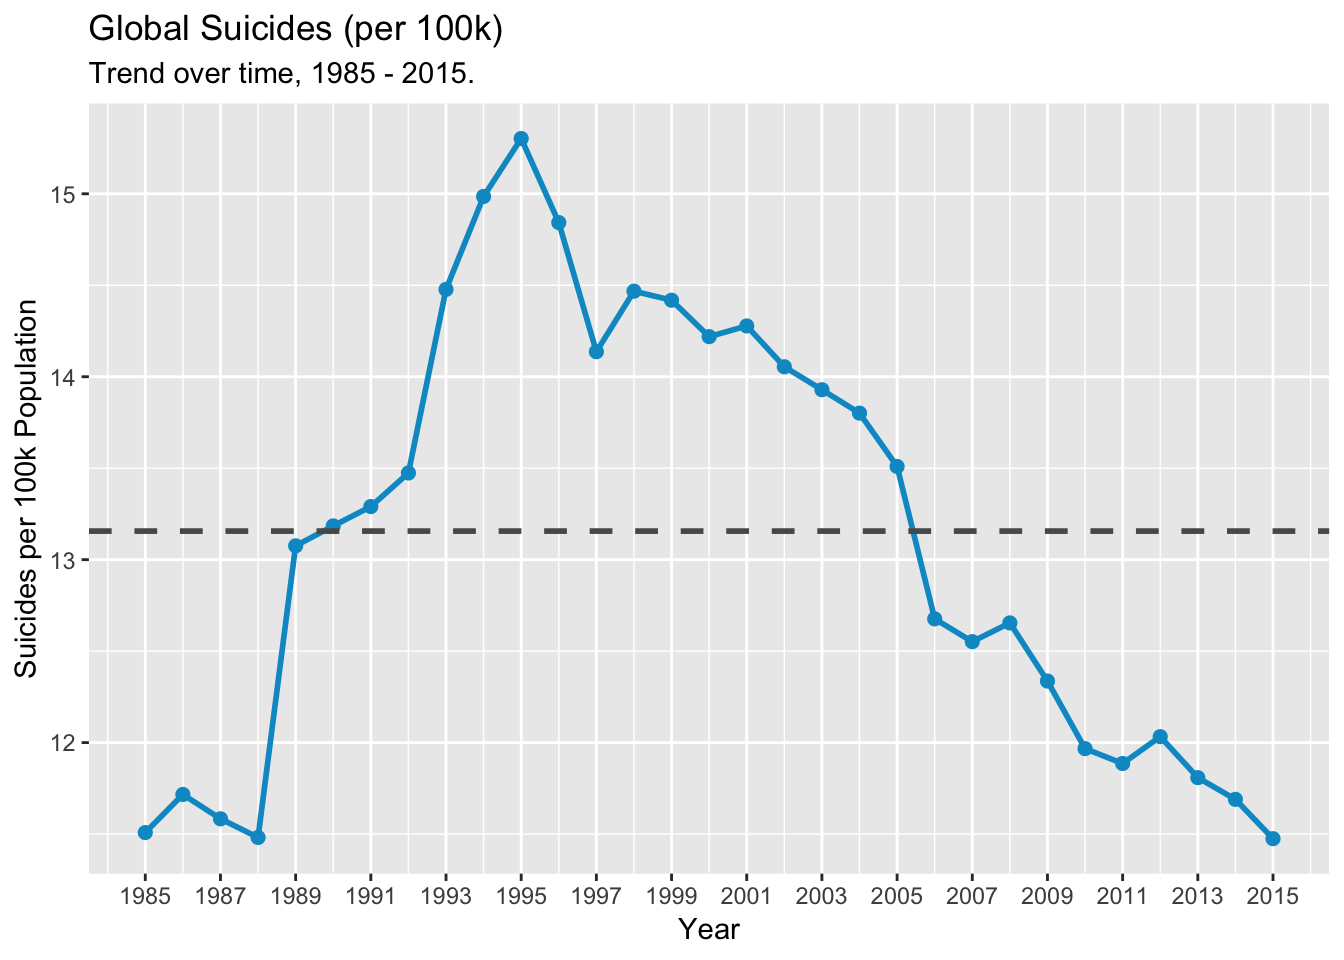
\includegraphics{suicides_files/figure-latex/unnamed-chunk-2-1.pdf}
\emph{Abbildung 1: Suicides per 100k per Year. Gestrichelte Linie ist
der globale Durchschnitt.}


\end{document}
